\documentclass[handout]{beamer}

\usepackage{fontspec} 
% \usepackage{lsp-makros}
\useoutertheme{lsp}

\usepackage{lsptitle}

\def\two@digits#1{\ifnum#1<10 0\fi\number#1}
\def\mytoday{\two@digits{\number\day}.\two@digits{\number\month}.\number\year}


\usepackage{xspace,multicol}
\newcommand{\latex}{\LaTeX\xspace}
\usepackage{tikz}


\newcounter{lastpagemainpart}
\footnotesep0pt
\renewcommand{\footnoterule}{}
\usefootnotetemplate{
  \noindent
  \insertfootnotemark\insertfootnotetext}

\let\beamerfn=\footnote
\renewcommand{\footnote}[1]{%
\let\oldfnsize=\footnotesize%
\let\footnotesize=\tiny%
\beamerfn<\thebeamerpauses->{#1}%
\let\footnotesize=\oldfnsize}


\date{\today}

\usepackage{eurosym}  
 
\renewcommand{\centerline}[1]{\hfill#1\hfill\hfill\mbox{}}


\title{\mbox{Linked Interlinear Examples}}
% \institute{FU Berlin}
\author[S. Nordhoff]{Sebastian Nordhoff}



\begin{document}
\lspbeamertitle
  
\frame{
    \frametitle{Books}
    
\includegraphics[width=2cm]{alor.png}
    \hfill
    
\includegraphics[width=2cm]{mauwake.png}
    \hfill
    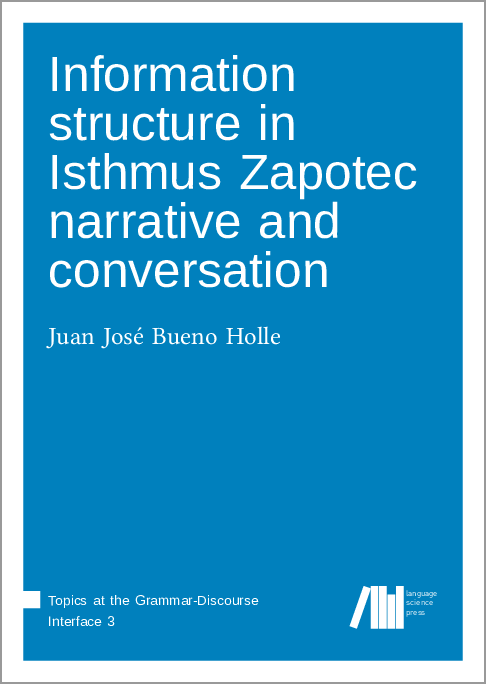
\includegraphics[width=2cm]{zapotec.png}
    \hfill
    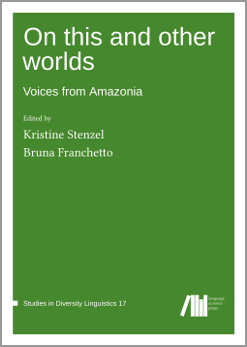
\includegraphics[width=2cm]{amazon.png}\\
    
\includegraphics[width=2cm]{komnzo.png}
    \hfill
    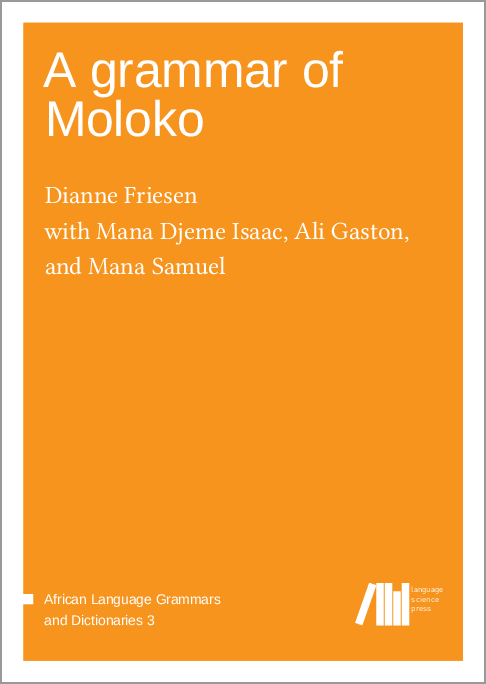
\includegraphics[width=2cm]{moloko.png}
    \hfill
    
\includegraphics[width=2cm]{pichi.png}
    \hfill
    
\includegraphics[width=2cm]{rapanui.png}
 }
 
 
\frame{
\frametitle{Interlinear examples}
    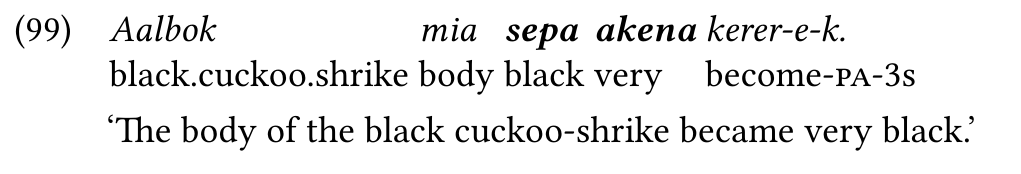
\includegraphics[width=10cm]{cuckooshrike.png}
 }
 
 
 
 
\frame{
\frametitle{Interlinear examples:\\ linked sentences}
    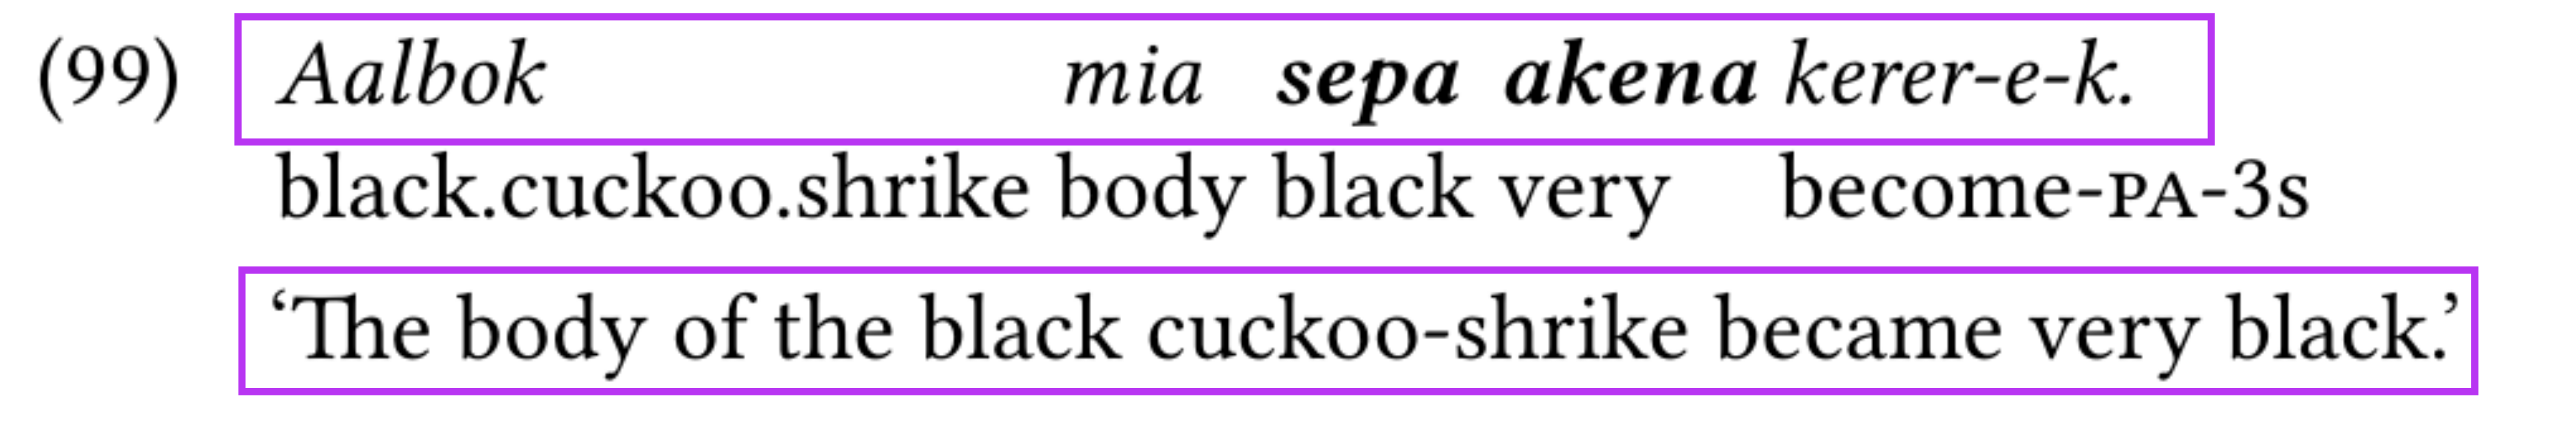
\includegraphics[width=10cm]{cuckooshrikes.png}
 }
 
 
 
\frame{
\frametitle{Interlinear examples:\\ linked words}
    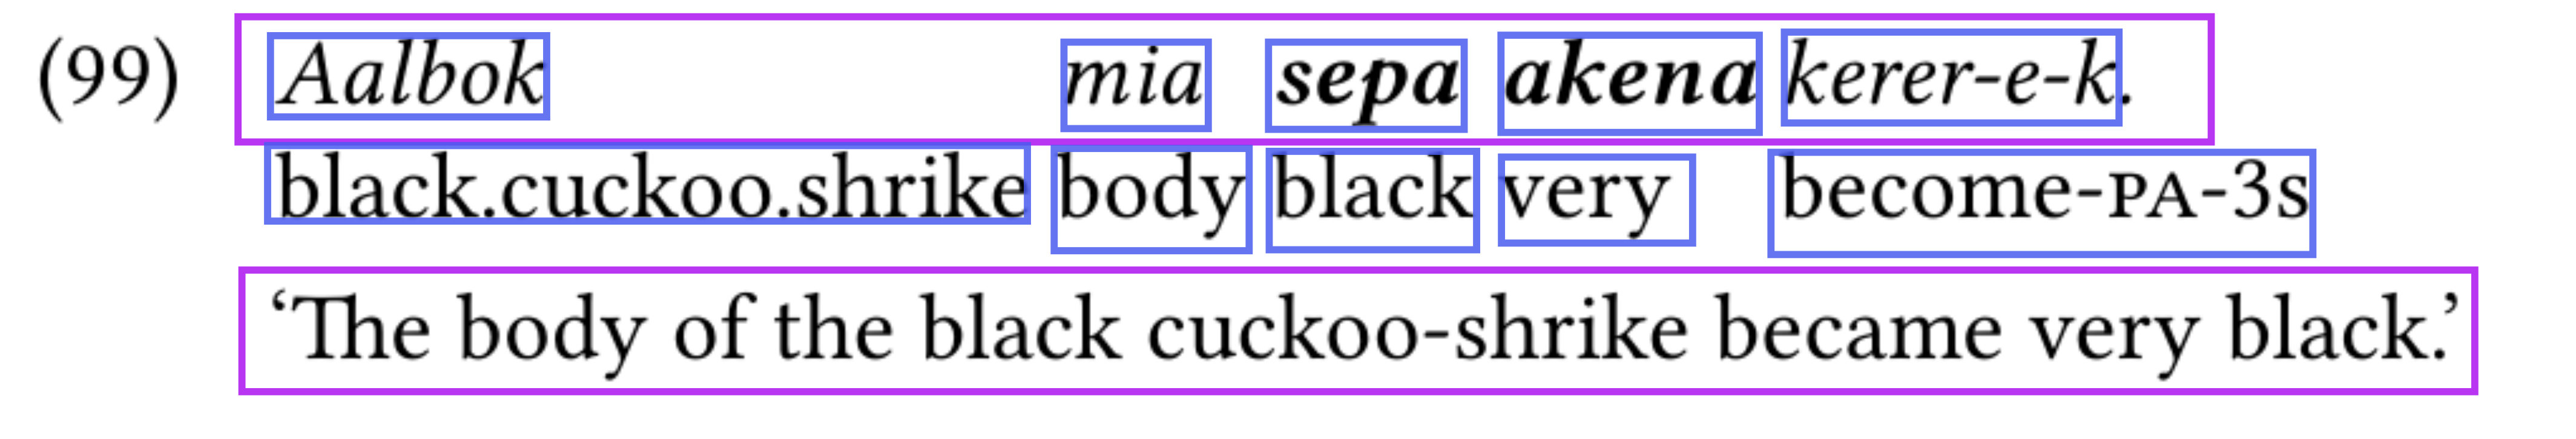
\includegraphics[width=10cm]{cuckooshrikew.png}
 }
 
 
 
\frame{
\frametitle{Interlinear examples:\\ linked morphemes}
    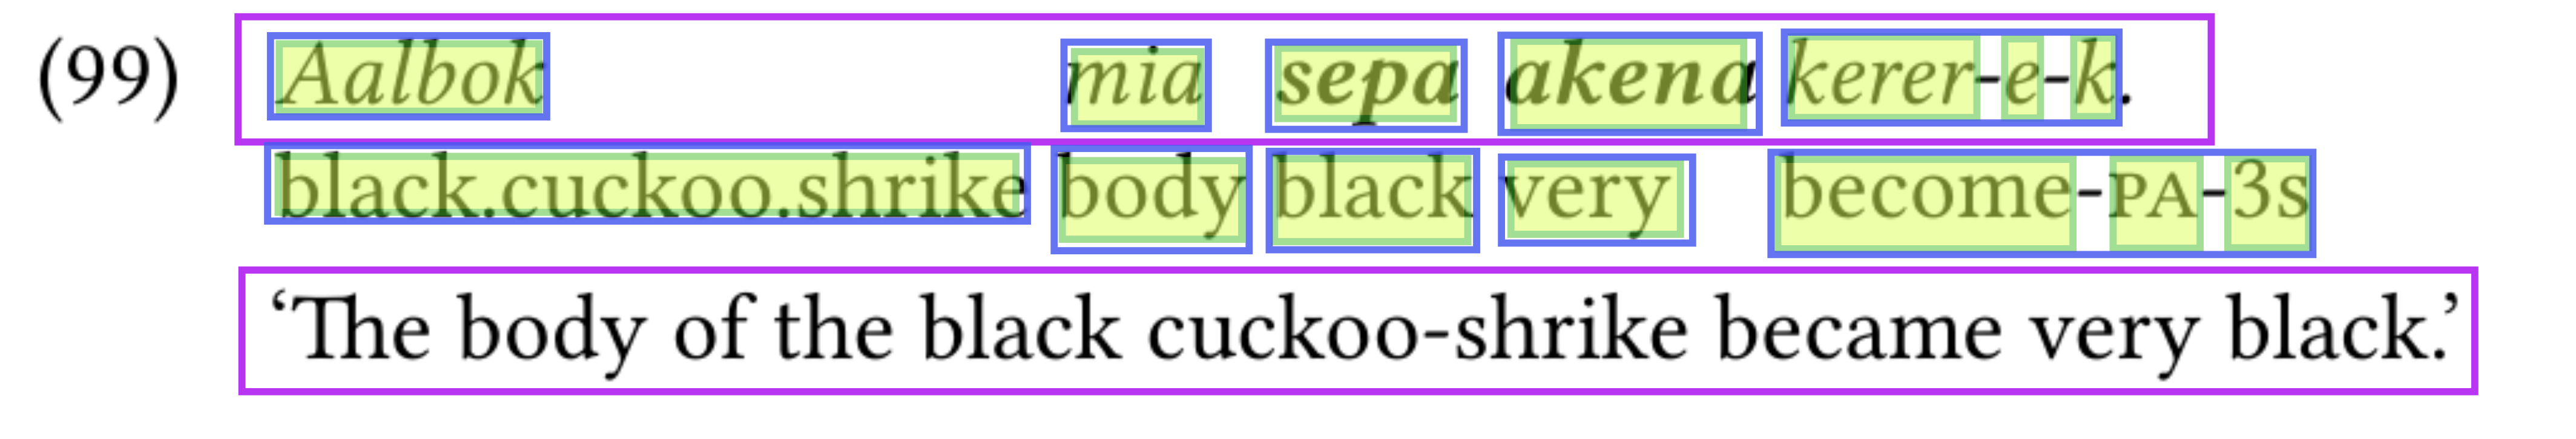
\includegraphics[width=10cm]{cuckooshrikem.png}
 }
 
 
\frame{
\frametitle{Interlinear examples:\\ linked concepts}
    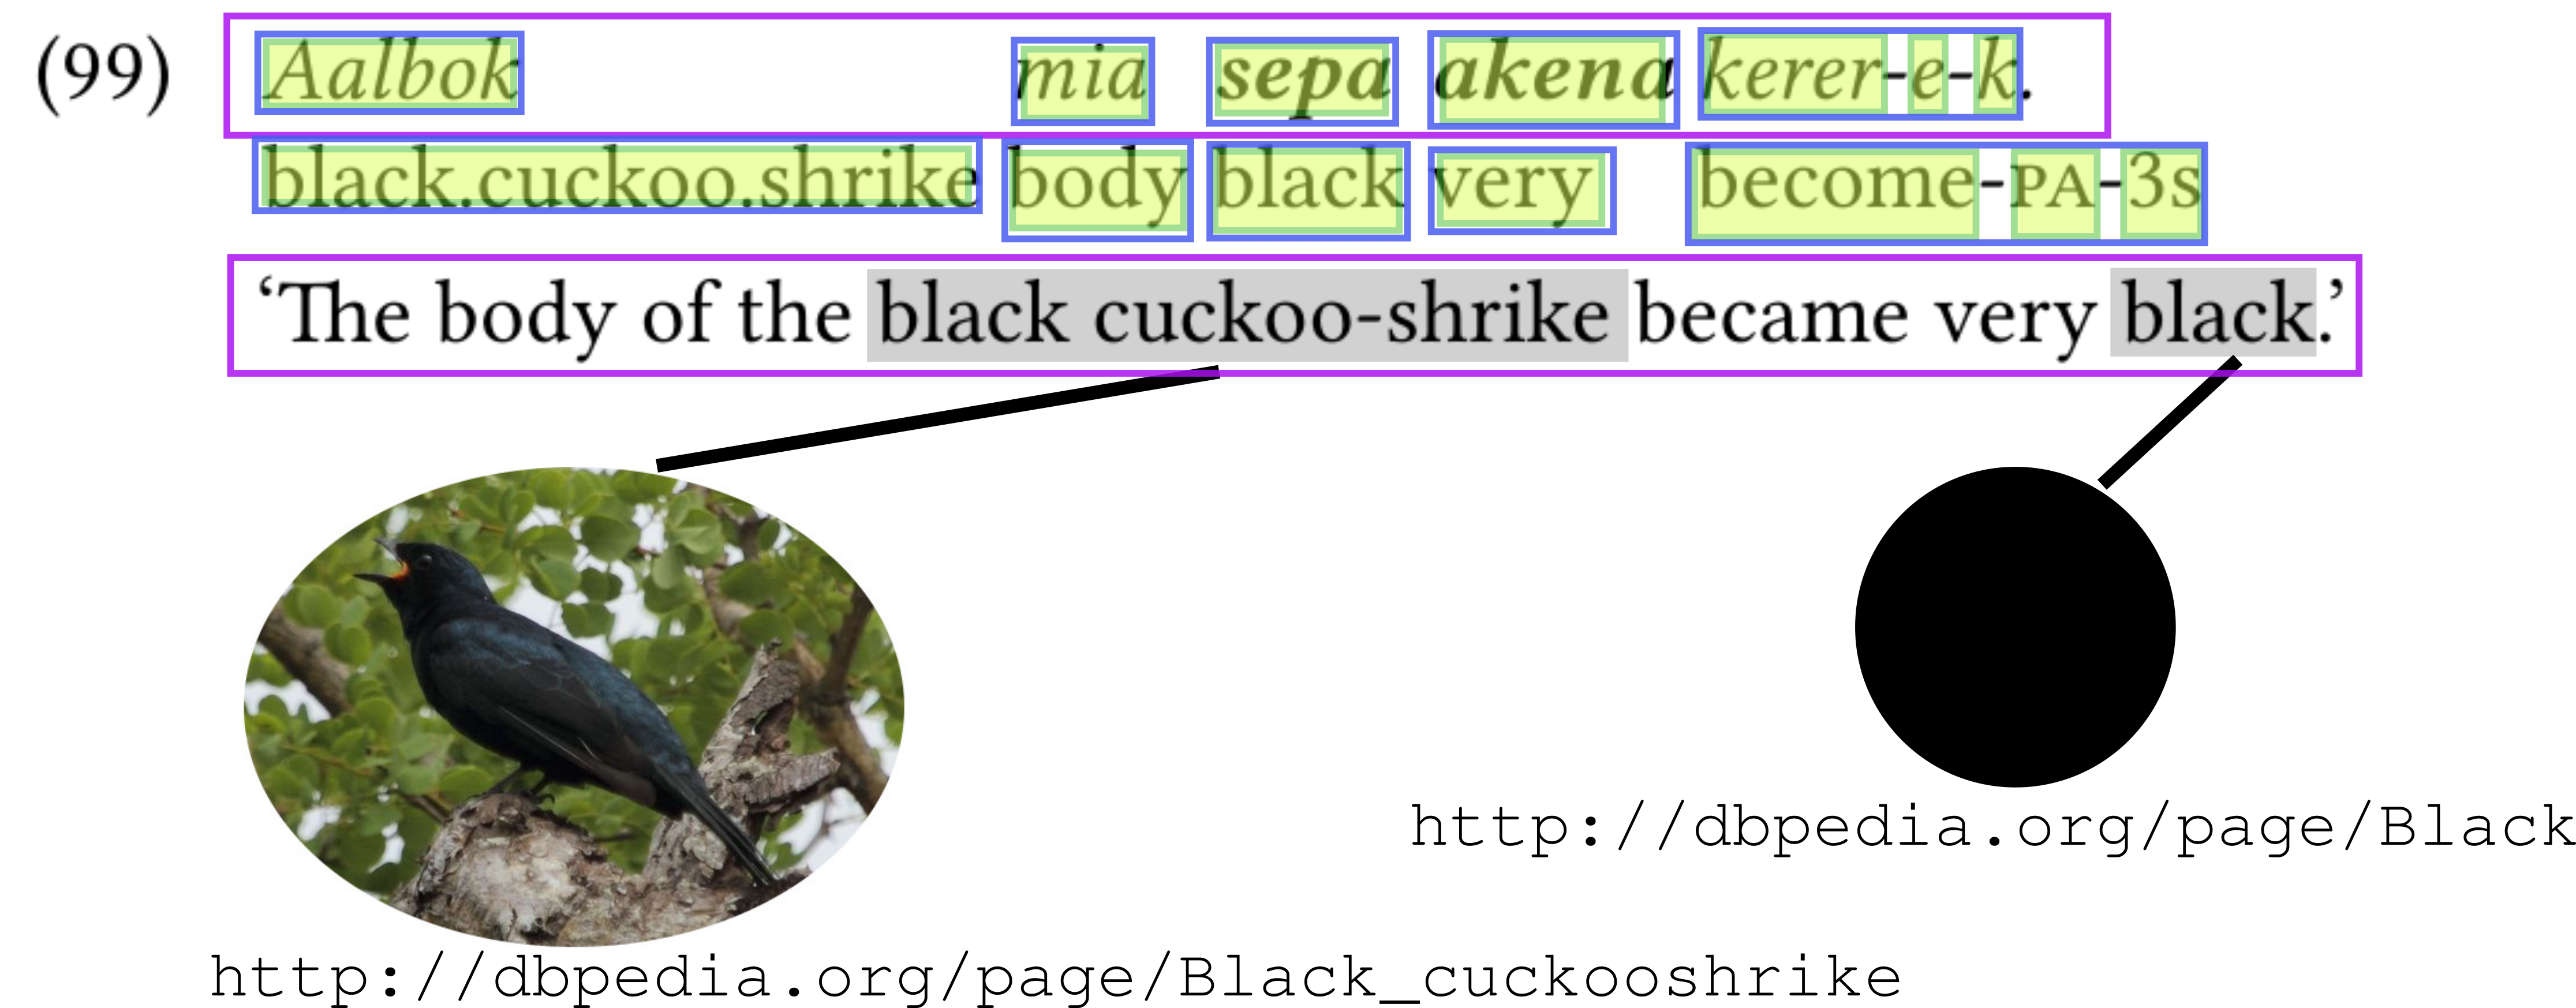
\includegraphics[width=10cm]{cuckooshrikelink.png}
 }
 

 
 
 
 
\frame{
    \frametitle{{\LaTeX} source}    
    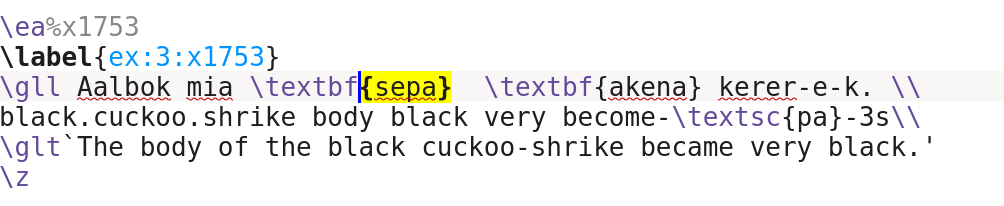
\includegraphics[width=10cm]{gll.png}
  \begin{itemize}
    \item Parsing and mapping of first and second line
    \item Entity recognition on third line
    \item 15\,000 vanilla examples available from 51 different books
  \end{itemize}
    }

    
    
 
\frame{
    \frametitle{LLOD modeling}    
  \begin{itemize}
 \item what is the precise relation between sentences, words, morphemes? 
%  \item how to handle separators (- for affixes, = for clitics)?
 \\
 \item hosting
%  \item content negotiation
 \item update strategies
 
 
 \item existing resources:
 
 \begin{itemize}
   \item 
 \texttt{extractgll.py}, outputs JSON
 \item \url{https://github.com/Glottotopia/exbase/tree/master/data/langscibooks}
 \item Another 15\,000 examples available from the Creole language database APiCS
 \end{itemize}

  \end{itemize}
    }

 
\end{document}
